%! Author = Vova
%! Date = 13.07.2021

% Preamble
\documentclass[11pt]{article}


% Packages
\usepackage{amsmath}
\usepackage{hyperref}
\usepackage{polyglossia}
\usepackage{graphicx}
\usepackage{babel,blindtext}
\usepackage{subfig}
\usepackage{iftex}
\usepackage{xcolor}
\usepackage{amssymb}
\usepackage{adjustbox}
\usepackage[normalem]{ulem}
\usepackage{amsfonts}

% Language and Font settings

% Kurale
% New Standard Old
\setdefaultlanguage{russian}
\setmainfont[Ligatures=TeX]{Kurale}
\newfontfamily\cyrillicfont{Kurale}

% Author, date
\title{Описание программной части робота-художника}
\author{Латыпов Владимир Витальевич}
\date{\today}

% Graphics settings
\graphicspath{{../images/}}

% Document
\begin{document}
    \maketitle
    \newpage
    \tableofcontents
    \newpage

    \section{Формулировка задачи}\label{sec:formulating_task}

    Для того, чтобы робот-художник нарисовал что-либо, ему нужно предоставить данные в определённом формате, а именно — не набор пикселей,
    как требуется для показа на мониторе, а набор «мазков»: это связано с конструкцией самого робота.

    Мазки решено было представлять в виде \href{https://en.wikipedia.org/wiki/B\%C3\%A9zier_curve}{кривых безье} второго порядка (то есть квадратичных), к которым добавлены параметры «толщина» и «цвет».
    (сама кривая задаётся тремя точками на плоскости)

    Но на вход подаются рисунки не в векторном, а в растровом формате.
    Найти такую комбинацию мазков, которая бы лучше всего соответствовала картине/изображению — задача нетривиальная, имеющая множество решений.

    Конечно же, я выбрал решать задачу самостоятельно, а не использовать готовые библиотеки.

    \section{Описание программы в общих чертах}\label{sec:general_description}
    Таким образом, решено было использовать эвристические алгоритмы оптимизации:
\href{https://en.wikipedia.org/wiki/Simulated_annealing}{Генетический алгоритм} и \href{https://en.wikipedia.org/wiki/Simulated_annealing}{Симуляция отжига}.
Подробное описание алгоритмов, моей их реализации и улучшений представлено в секции \ref{sec:opimization_algorithms}.

\subsection{Представление «решения»  — набора мазков}
Программа работает с последовательностями мазков, находя лучшую из них.
Однако, чтобы алгоритм оптимизации работал с ними, наборы мазков должны быть представлены в виде векторов в $\mathbb{R}^n$.
Формат данных в «геноме» таков:

\begin{figure}[h]
    \centering
    \adjincludegraphics[width=0.7\textwidth, clip, trim={0.15\width} {0.7\height} {0.15\width} {0.125\height}]{genome_contents_table.pdf}
    \caption{Схема хранения генома}
    \label{fig:genome_contents_table}
\end{figure}


, где $p_{n_x} ~\&\&~ p_{n_y}, n \in \{ 0, 1, 2 \}$ — координаты направляющей точки под номером n (из всего 3 у каждого мазка),
а \textit{width}  — толщина мазка.

Здесь нет параметра  «цвет».
Причина объяснена в разделе: \ref{subsec:color_in_genome}.

\subsection{Задание функции ошибки}
Чтобы решить задачу алгоритмом оптимизации, нужна некая метрика — функция, которая будет определять степень «неподходящести» данного ей решения.
Именно она будет передаваться алгоритму оптимизации.
В нашем случае вычисление ФО включает в себя растеризацию мазков (отображение их на изображении) и вычисления, производящие сравнения полученного результата с желаемым.
Функцию ошибки необходимо задать таким образом, чтобы она отражала качество полученной комбинации мазков,
причём в любой точке направление её уменьшения соответствовало направлению улучшения результата.
За основу была выбрана \href{https://en.wikipedia.org/wiki/Mean_squared_error}{MSE} (Mean Square Error):

\begin{equation}\label{eq:equation}
    MSE = \frac{1}{width \cdot height} \cdot \sum_{y = 0}^{y < height} { \sum_{x = 0}^{x < width} { \sum_{c \in  \left\{ r, g, b \right\} } { \left( {\overrightarrow {rendered_{x, y}}}_c - {\overrightarrow{original_{x, y}}}_c\right)^2 }}}
\end{equation}

MSE — универасльная мертрика для схожести изображений, она повсеместно используется при работе с ними.
Но в нашем случае, о чём свидетельствует практика, целесообразно добавить в ФО компоненту, «наказывающую» наложение мазков и пустые, ничем не закрашенные места.

Первое улучшение очевидно — при прочих равных лучше ситуация, при которой та же картина достигнута с меньшим использованием краски
(а если не вводить эту компоненту, наложено в найденном решении может быть сразу много (> 2) мазков в одной точке).
Если нет разницы, зачем переплачивать?

С теоретической точки зрения может быть непонятна надбавка за пустоты: ведь если место пустое, оно и так не даёт оптимальное MSE.
Однако на практике пусто́ты недостаточно быстро и полно покрываются (особенно — на ускоренном режиме) без этой надбавки.

Таким образом, функция ошибки сделана так, чтобы максимально стимулировать правильно распределение мазков.

\subsection{Растеризация мазков}\label{subsec:rasterization}
Имея мазок, заданный в виде трёх точек на плоскости, толщины и цвета, нужно уметь его отобразить его на «холсте», то есть в виде набора пикселей.
Это нужно, чтобы подсчитать функцию ошибки для заданного набора мазков,
причём так, чтобы результат максимально соответствовал мазку, рисуемому роботом.
В качестве достаточно точной модели описания такого мазка возьмём круглую кисть, перемещающуюся по заданной траектории.
Есть много способов произвести растеризацию.
Нужно выбрать тот, который будет производительным и в то же время максимально близким к реальному мазку.

Самый простой — для некоторого количества точек на кривой Безье (с достаточно маленьким шагом, примерно один пиксель) проводим вертикальную линию: вверх на width и  вниз — тоже.
Это даёт высокую производительность и сносно выглядит на участках, близких к горизонтальным, но результат, полученный таким способом, очень далёк от реальности на вертикальных участках:
\begin{figure}[h!]
    \centering
    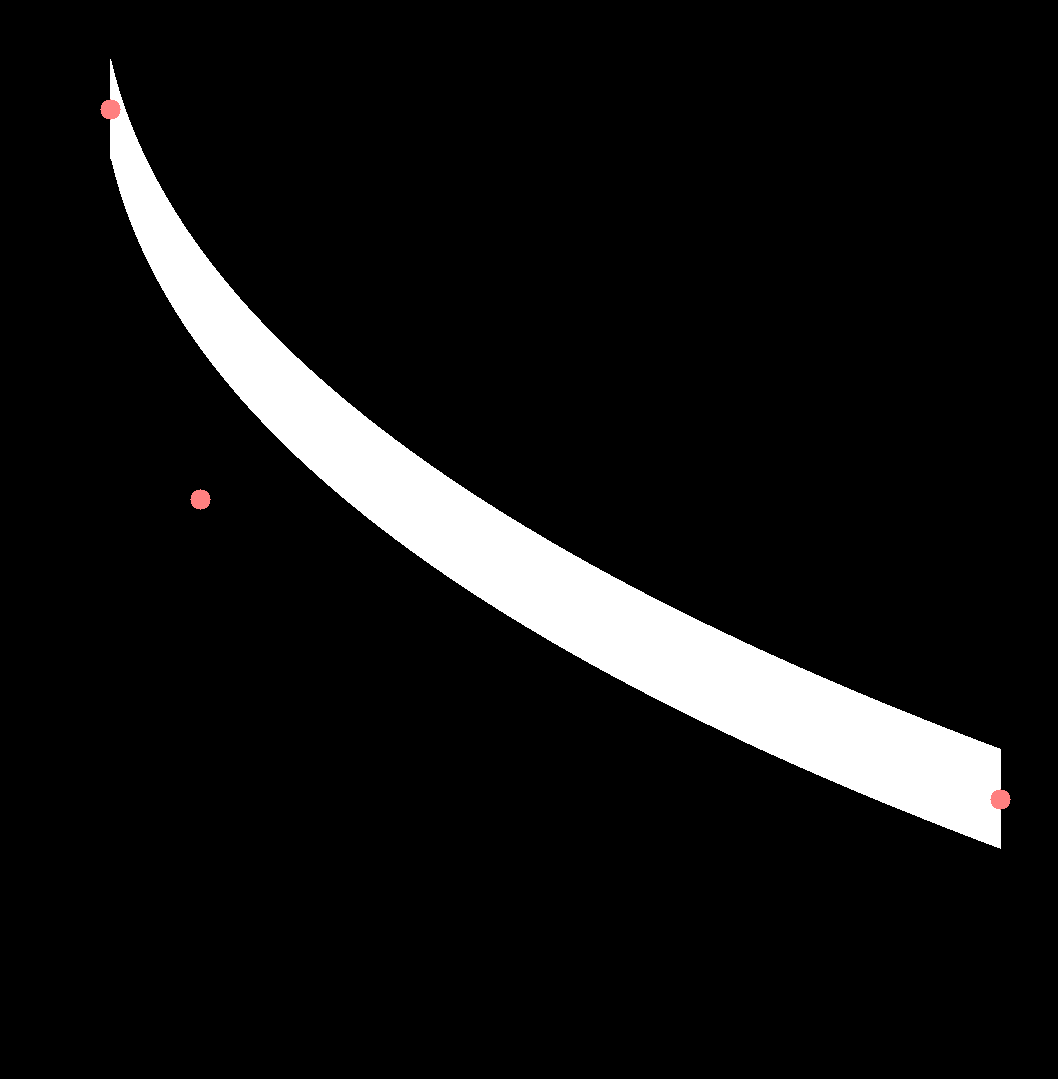
\includegraphics[width=0.75\textwidth]{stroke_vertical.png}
    \caption{(Красным обозначены точки, задающие кривую)}
    \label{fig:vertical_stroke}
\end{figure}
\begin{figure}
    \centering
    
\includegraphics[width=0.75\textwidth]{one_stroke.png}
    \caption{Иногда такой способ добавляет свой шарм}
    \label{fig:pretty_vert_stroke}
\end{figure}

Есть разные способы избавиться от этих недостатков, сохраняя максимальную производительность.
Например:
\begin{itemize}
    \item Совмещать горизонтальные и вертикальные полосы
    \item Проводить полосы перпендикулярно направлению кривой в данной точке
\end{itemize}
В каждом из них будут наблюдаться пустые места, полости, что недопустимо.

Ультимативным же способом является подражание реальной жизни: «проведение» круглой «кистью» по экрану.
То есть берутся точки на кривой на небольшом расстоянии друг от друга, и с центром в каждой из них рисуется круг радиусом width.
Однако в таком случае каждая точка, попадающая в мазок обрабатывается много раз (для близких кругов), что значительно замедляет рендерниг.
Если же увеличить шаг, этой проблемы можно частично избежать, но мазок стал бы неровным.
При маленьком шаге это выглядит так:
\begin{figure}[h!]
    \centering
    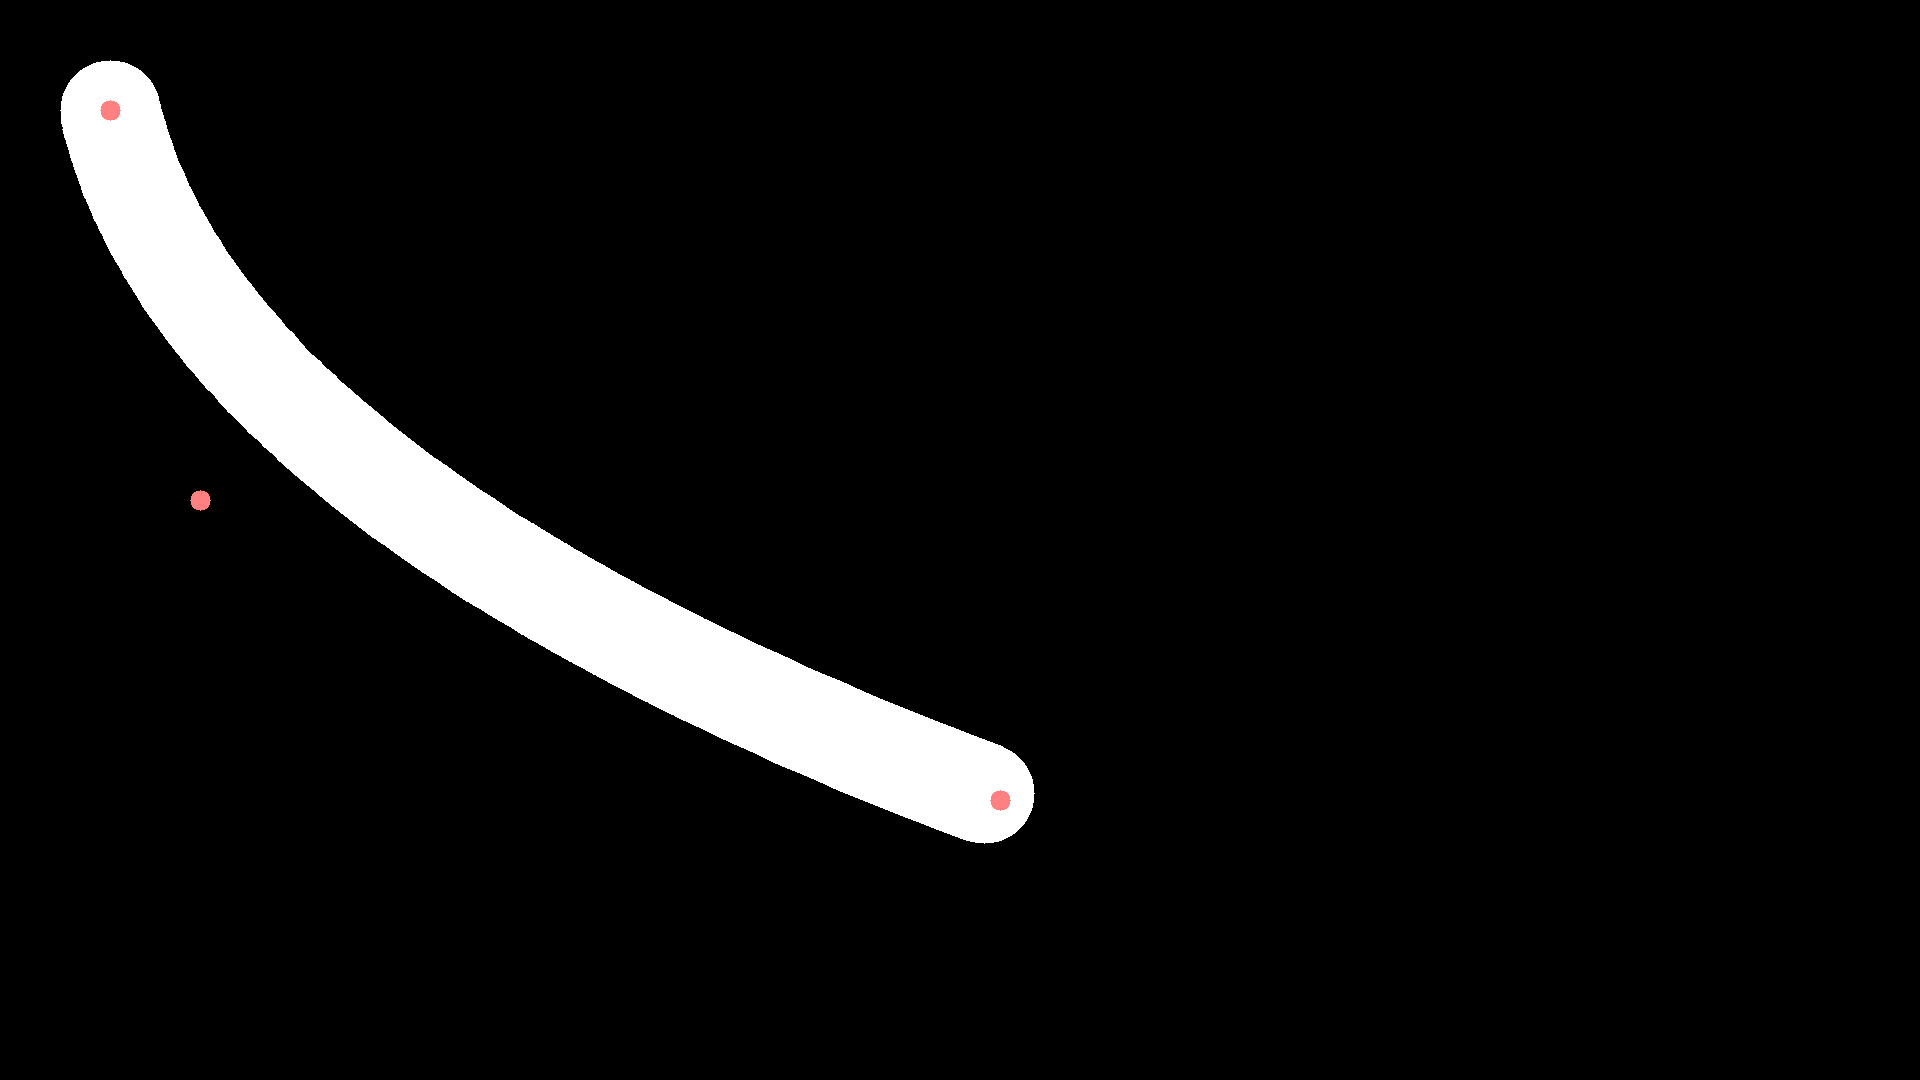
\includegraphics[width=0.75\textwidth]{stroke_smooth.png}
    \label{fig:smooth_stroke}
\end{figure}

В будущем планируется улучшить алгоритм для ускорения растеризации при почти том же качестве.
Рассматриваются варианты:
\begin{itemize}
    \item Заменить круглую кисть на также гладкую, но с более медленным закруглением с дальней от вектора кривой в данной точке стороны, поворачивая кисть соответствующим образом:
    \begin{figure}[h!]
        \centering
        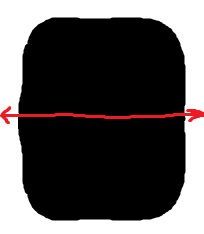
\includegraphics[width=0.75\textwidth]{modern_brush.png}
        \caption{(красным обозначено направление вектора кривой)}
        \label{fig:modern_brush}
    \end{figure}
    Такое изменение поможет уменьшить артефакты при увеличении шага между точками на кривой, то есть позволит сделать шаг больше, ускорив процесс.

    \item Автоматически разбивать мазок на «полигоны».
                Для этого нужно пройтись по кривой и с некоторым шагом (уже побольше, чем раньше),
                отметить для каждой рассматриваемой точки на прямой, содержащей её и перпендикулярной текущему направлению, точки в обе стороны от неё на расстоянии width.
                Каждая из них добавляется в соответствующий стороне в порядке обхода список.
                Потом полигоны, полученные из соседних точек на кривой и соответствующим им вынесенным точкам, заливаются нужным цветом.
                На концах же мазка рендерятся круги.

    \begin{figure}[h!]
        \centering
        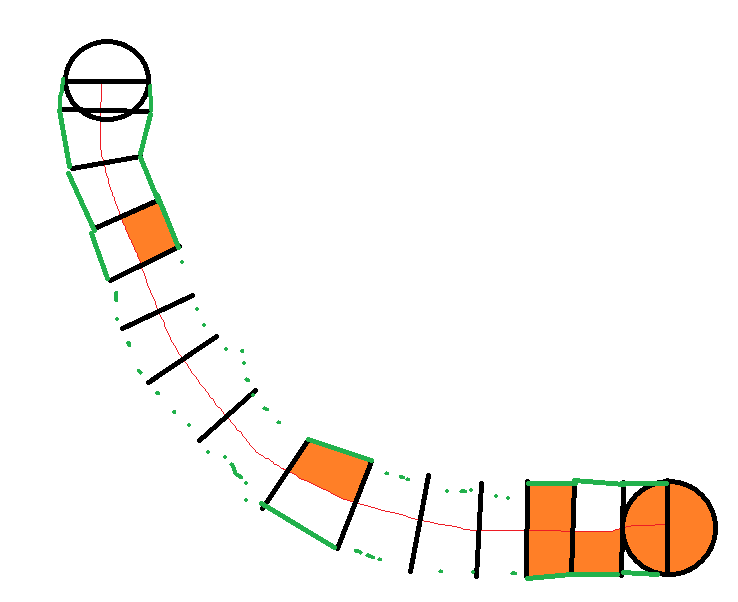
\includegraphics[width=0.75\textwidth]{polygonal_stroke.png}
        \caption{Схема полигональной разбивки мазка}
        \label{fig:polygonal_stroke}
    \end{figure}

    При использовании этого метода никакая существенная часть пикселей мазка не обрабатывается по много раз, что говорит о высокой эффективности алгоритма.
    Поэтому я собираюсь внедрить такой метод в ближайшее время.
\end{itemize}

Что же касается совместимости с видеокартой,
для круга и модифицированной кисти понятно, как определить bouding-box,
и понятно, как по координатам пикселя быстро определить, принадлежит ли он этому примитиву.
А рендеринг полигонов производится аппаратно.

Подробнее про внедрение видеокарты можно почитать в разделе \ref{subsec:move_graphics_to_videocard}.


\subsection{Учёт цвета при оптимизации}\label{subsec:color_in_genome}

\subsubsection{Знание цвета при рендеринге необходимо}
Цвет является обязательным параметром мазка, без которого непонятно, как его растеризовать.
Но значит ли это, что цвет обязательно должен быть одним из параметров алгоритма оптимизации?
Конечно же, нет.

\subsubsection{Определение цвета по положению при подсчёте ФО}
Во-первых, цвет может быть легко определён, зная положение.
Самый простой способ — найти среднее арифметическое цветов пикселей.
Мы автоматически получим минимальное MSE,
так как для каждой из цветовых компонент соответствующая часть MSE — сумма квадратичных функций (для каждого пикселя),
причём «с ветвями вверх» (так как на бесконечностях она уходит в $+ \infty$), которая имеет одну точку с нулевой производной — как раз в среднем арифметическом:

\begin{equation}
    \begin{gathered}
        MSE_c(value_c) = \sum_{pixel \in {pixels}} \bigg(value_c - pixel_c\bigg)^2 \\
        \Rightarrow \\
        MSE_c'(value_c) = 2 \cdot \left( \lVert pixels \lVert \cdot value_c - \sum_{pixel \in {pixels}}  pixel_c \right)
    \end{gathered}
\end{equation}
, где $pixel_c$ — значение канала $c$ пикселя $pixel$.

То есть у MSE достигается производная ноль в этой точке:
\begin{equation}
    MSE_c'(value_c) = 0
    \Longleftrightarrow
    value_c = \frac{\sum_{pixel \in {pixels}}  pixel_c}{\lVert pixels \lVert} = \overline{pixel}
\end{equation}
Следовательно, больше нигде ноль не достигается, так как функция квадратичная.
Более того, это минимум, так как функция — «ветви кверху».

\subsubsection{Фиксированный цвет в зонах}
Во-вторых, при делении на зоны все пиксели, относящиеся к данной зоне, имеют строго заданный цвет.
Подробнее об этом читать в секции \ref{subsec:applying_zoning}.


\subsection{Разделение картины на зоны}\label{subsec:applying_zoning}
Известно, что время оптимизации до заданного качества очень сильно увеличивается при увеличении количества параметров.
Причём существенно более быстро, чем линейно.
Следовательно, можно получить выгоду, разделяя эти параметры каким-то образом и оптимизируя группы по отдельности.
Вопрос в том, в каких случаях это делать можно, а в каких — нет.

Надо понимать, что нельзя независимо опт. ближайшие мазки (пояснить)
Однако дальние мазки — нет
Если мутация затрагивает большое количество мазков из разных сторон изображения, «картина» для функции ошибки очень зашумлена (пояснить)

% TODO: продолжить, рассказать про совмещение прямоугольников (наложение, заполнение крестов), зоны svg

\subsection{Сортировка мазков перед выпуском}\label{subsec:stroke_sorting}

\subsubsection{Сортировка по территориальному признаку}

\subsubsection{Оптимальная расстановка цветов}



    \section{Технические аспекты}\label{sec:tecnical}
    \subsection{Основное}\label{subsec:major}
Программа написана на языке программирования C++(так как требовалась максимальная скорость), сборка осуществляется с помощью CMake.
Проект можно скомпилировать под Windows (компилятор MSVC) и под Linux (тестировалось на g++-10).

Код хранится в \href{https://github.com/donRumata03/Painter}{guthub-репозитории (кликабельно)}.

\subsection{Библиотеки}\label{subsec:libs}

\subsubsection{OpenCV}
Для работы с изображениями используется OpenCV, но не модуль машинного обучения, а лишь примитивные операции с изображениями:
прочтение из популярных форматов, сохранение в них, хранение и копирование матрицы пикселей и т.д.

\subsubsection{Pythonic}
Для работы проекта также необходима библиотека «\href{https://github.com/donRumata03/pythonic}{pythonic}»: она написана мной, подключается также через CMake.
Она отвечает за базовые функции и структуры данных.
Я использую её во всех более или менее крупных проектах на C++.
В ней на данный момент есть:
\begin{itemize}
    \item Простые вспомогательные функции для работы со строками, контейнерами, форматированного вывода
    \item Вызов питоновской библиотеки matplotlib для построения графиков
    \item Базовые алгоритмы наподобие бинарного поиска и дерева отрезков
    \item Функционал для работы со временем, в том числе — анализатор последовательных запусков процесса
    \item Платформонезависимая работа с кодировками и файловыми системами
    \item Примитивы для вычислительной геометрии
    \item Функции для работы со статистикой
    \item Многомерный шаблонный массив с количеством измерений, изменяемом в run-time
    \item Сглаживание функций и построение примерной функции распределения в пространстве с заданной размерностью по набору sampl-ов с помощью гауссовых ворот
    \item Функционал для работы с многопоточностью, в том числе — thread pool, умеющий снимать нагрузку с ожидающих потоков с помощью std::condition\_variable.
\end{itemize}

\subsubsection{lunasvg}
Для работы с SVG используется библиотека \href{https://github.com/sammycage/lunasvg}{lunasvg}.
P. S. У этой библиотеки отличный автор, он изучает проекты, в которых библиотека используется, и пишет рекомендации о best prictice её использования.

\subsubsection{PowerfulGA}
Функционал по методам оптимизации реализован мной и вынесен в отдельную репозиторию: \href{https://github.com/donRumata03/PowerfulGA}{click}
(там не только Генетический алгоритм, как можно было подумать из названия, но и симуляция отжига, градиентный спуск, метод Ньютона;
многие другие алгоритмы планируются быть добавленными)
Более подробное описание в секции $\longrightarrow$ \ref{sec:opimization_algorithms}

    \section {Алгоритмы оптимизации}\label{sec:opimization_algorithms}
    \subsection{Общий принцип ГА}\label{subsec:ga_general_principles}
Идея работы Генетического алгоритма заимствована у природы.

Точно также, как в ходе эволюции происходит появление оптимального организма для заданных условий,
в ходе работы алгоритма ищется набор параметров функции, при котором фитнесс-функция максимальна.

В природе тот, кто лучше приспособлен к окружающей среде, в большей степени получает доступ к размножению (с помощью различных механизмов),
а при размножении новая особь наследует признаки каждого из родителей.

Это позволяет именно лучшим чертам, по каким-либо причинам появившихся у особей, переходить в следующее поколение.
Эти черты появляются через мутации — небольшие случайные изменения в геноме.

Из принципа работы можно понять, что алгоритм \href{https://en.wikipedia.org/wiki/Heuristic_(computer_science)}{эвристический}: сложно доказать его сходимость или что-либо гарантировать с вероятностью 100\%.
Зато \href{talgat.org/news/wp-content/uploads/2018/08/112.pdf}{исследования} показывают, что именно этот алгоритм даёт лучшие результаты для самых сложных функций.
В разделе \ref{subsubsec:hazing}, какие меры предпринимаются, чтобы не дать алгоритму попасть в локальный минимум, не добравшись до глобального.

\subsection{Термины}\label{subsec:ga_principles}
Набор параметров представляется в виде \textit{«генома»} — некой структуры данных, содержащей информацию об этом наборе.
\textit{Особь} — в контексте алгоритма будет использоваться в качестве синонима к геному.
Геном состоит изх \textit{генов} — каждый из них содержит информацию о каком-либо признаке (в случае природы) или параметре (в случае ГА).

В каждый момент времени алгоритм работает с \textit{популяцией} — набором геномов.
Полный аналог популяции в природе.
Мутация — как и в реальной жизни — небольшое случайное изменение генома без строго определённого направления.

\subsection{Примерная последовательность действий ГА}\label{subsec:approx_ga_algo}
В общих чертах работа ГА выглядит так:

\underline{Инициализация}: Сгенерировать случайную популяцию, каждый ген каждого генома — в заданных пределах.

Затем — повторять, пока не закончится заданное количество итераций или не будет достигнуто требуемое значение фитнесс-функции:
\begin{enumerate}
    \item Посчитать фитнесс-функции для каждой из особей.
    Для большинства задач этот шаг занимает бо́льшую часть времени исполнения, поэтому нужно оптимизировать именно его, в частности — параллелизовать, запуская независимые вычисления на нескольких потоках.
    \item Каким-то образом отобрать особи на скрещивание
    \item Произвести скрещивание, получив «отпрысков» — часть нового поколения
    \item Сформировать новое поколение, используя, возможно, в разных пропорциях, различные источники геномов, а именно:
            \begin{itemize}
                \item Отпрысков, полученных на предыдущем шаге в результате скрещивания
                \item Лучшие особи из прошлой популяции
                \item Случайные особи —  чтобы не дать алгоритму сойтись раньше времени, попав в локальный минимум
                \item Возможно, результаты скрещивания особей в числе больше 2
            \end{itemize}
    \item Произвести мутации в некоторых особях этого поколения (лучшие из мутаций внедрятся в популяцию на следующих итерациях)
    \item Если алгоритм подходит к концу, добавить лучший геном из предыдущего поколения (чтобы он не подвергся мутации)
\end{enumerate}

\subsection{Авторские Модификации  в ГА}\label{sec:my_modifications}

Учитывая тот факт, что в большинстве задач, решаемых мною, бо́льшая часть вычислительного времени ($\gg 95\%$) используется для подсчёта функции ошибки, а не для маниппуляций с геномами
(это подтверждается результатами профайлинга).
То есть задача состоит в том, чтобы минимизировать количество подсчётов функции ошибки, даже ценой более долгой работы с геномами.

Первое изменение — я решил отказаться от дискретного кодирования геномов.
Для алгоритма по каждой переменной задан её диапазон.

Традиционный подход — разделить диапазон на $2^N$ частей и кодировать номер части в геноме как битовую последовательность из $N$ бит.
Для подсчёта функции ошибки этот номер перекодируется назад в соответствующую точку непрерывной величины.
Мутацей в данном случае является изменение случайного количества каких-то битов этого номера.
А скрещивание обычно происходит путём

Предварительное тестирование показало бо́льшую эффективность этого метода по сравнению с традиционным подходом, однако планируется провести тщательное тестирование (см. \ref{itm:testing_system})

\subsubsection{hazing\_percent: скорость сходимости}\label{subsubsec:hazing}
Соотношение элит
Нужно исследовать всю область поиска, для этого нужно не давать сразу огромный бонус при размножении и переходе в другое поколение за некоторое преимущество.
Так получится обеспечить развитие нескольких «очагов», внутри которых и будет происходить «шлифование» «идеи искать в этой области».
% TODO: Лучше описать это

Алгоритм реализован мной на языке C++, он хранится в GitHub репозитории \href{https://github.com/donRumata03/PowerfulGA}{https://github.com/donRumata03/PowerfulGA}.

    \section{Наблюдения}\label{sec:observations}
    \subsection{Неравенство зон}\label{subsec:inequality}
Когда я заметил, что зоны, на которые Adobe Illustrator делит изображение, могут очень сильно отличаться в размере (отношение площадей может достигать 1000 раз),
мне захотелось измерить это неравенство численно, чтобы при разработке нового алгоритма измерять его качество в том числе по этому параметру.
(понятно, что наличие зон слишком малого или слишком большого размера плохо сказывается на работоспособности алгоритма;
то же самое можно сказать и про узкие и длинные зоны, особенно — если )

Существует большое количество метрик, я решил выбрать основные из них:
\begin{itemize}
    \item Индекс Джини (вместе с кумулятивным графиком распределения дохода (также известен как \href{https://en.wikipedia.org/wiki/Lorenz_curve}{кривая Лоренца}))
    \item Процент «дохода» 1\% самых богатых от общего «дохода» (В случае зон вместо дохода используется занимаемая площадь).
    \item Процент самых богатых, имеющих в сумме 50\% от общего дохода.
\end{itemize}

Индекс Джини рассчитывается как отношение площади между кривой Лоренца и «линией равенства» к площади под линией равенства.
Иными словами, $G = \frac{A}{A + B}$ на этой схеме:

\begin{figure}[h!]\label{fig:lorenz_curve}
    \centering
    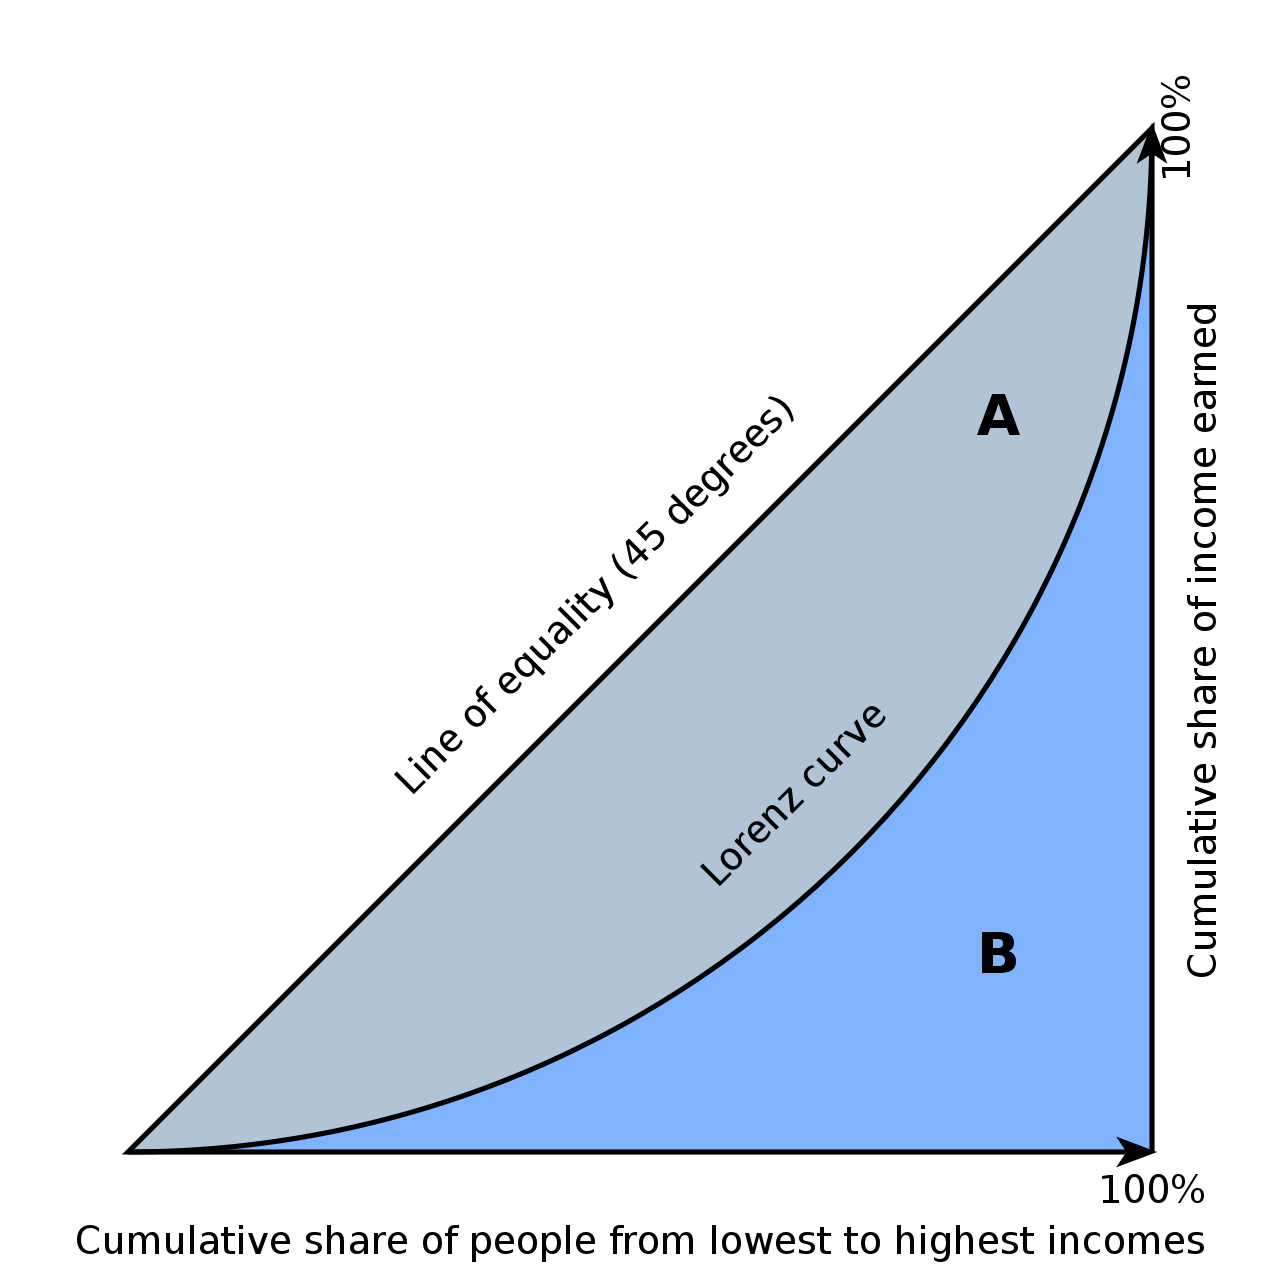
\includegraphics[width=0.75\textwidth]{typical_lorenz_curve.png}
    \caption{Типичная кривая Лоренца}
\end{figure}
Альтернативный способ посчитать коэффициент, использующийся в реализации:
\begin{equation}
    G = \frac{\sum_{i=1}^{n}  \sum_{j=i+1}^{n}  \left| y_i - y_j \right|}{n \cdot \sum_{i=1}^{n} y_i}
\end{equation}
Чем индекс выше, тем большее неравенство наблюдается в стране.
Более того, использование именно этой метрики позволяет комплексно оценить неравенство между анализируемыми объектами —
в отличие от рассмотрения процентов дохода заданного квантиля.


Результаты оказались впечатляющими:
\begin{itemize}
    \item $Gini\_index \approx 76\%$
    \item 1\% крупнейших зон покрывают ≈ 18\% изображения
    \item 6.25\% зон покрывают половину изображения
\end{itemize}

Так выглядит кумулятивный график распределения площади:
\begin{figure}[h!]\label{fig:cumulative_inequality_graph}
    \centering
    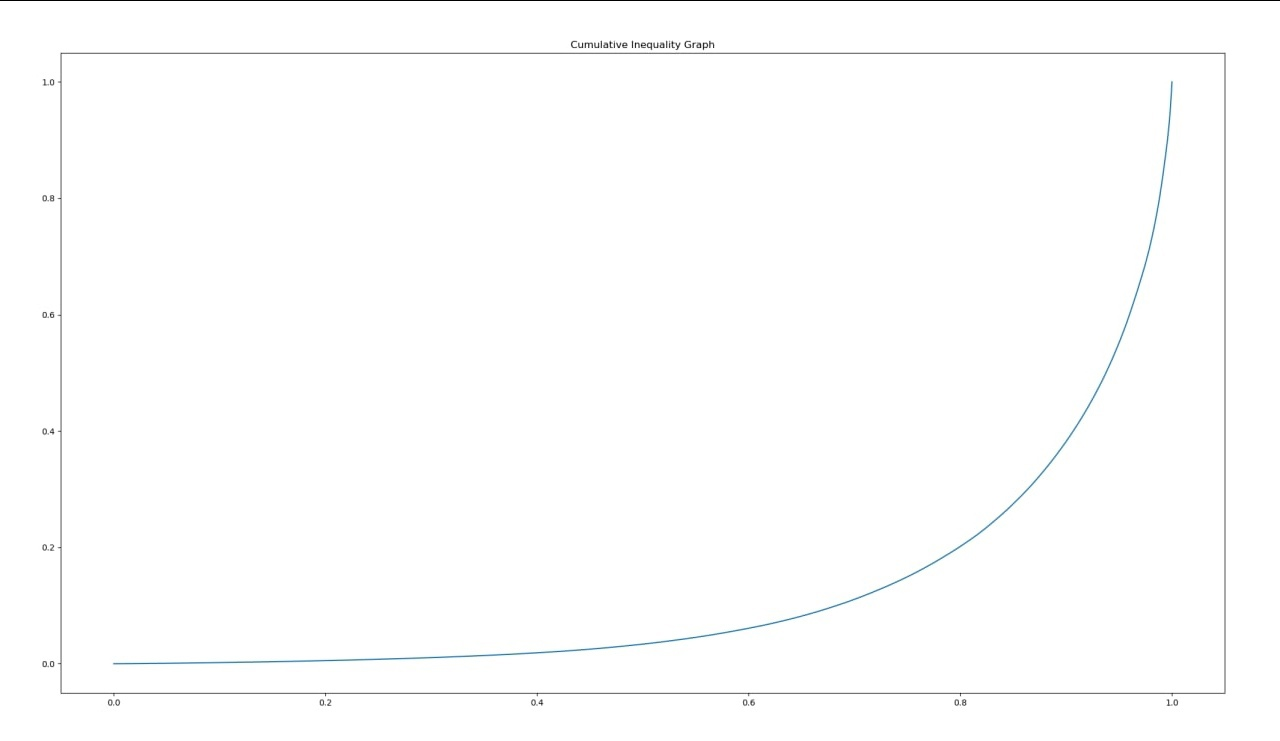
\includegraphics[width=0.75\textwidth]{cumulative_inequality_graph.jpg}
    \caption{Кривая лоренца для зон}
\end{figure}

Нетрудно заметить, что ни в одной стране мира нет такого неравенства, как среди зон:

\begin{figure}[h!]\label{fig:gini_index_world}
    \centering
    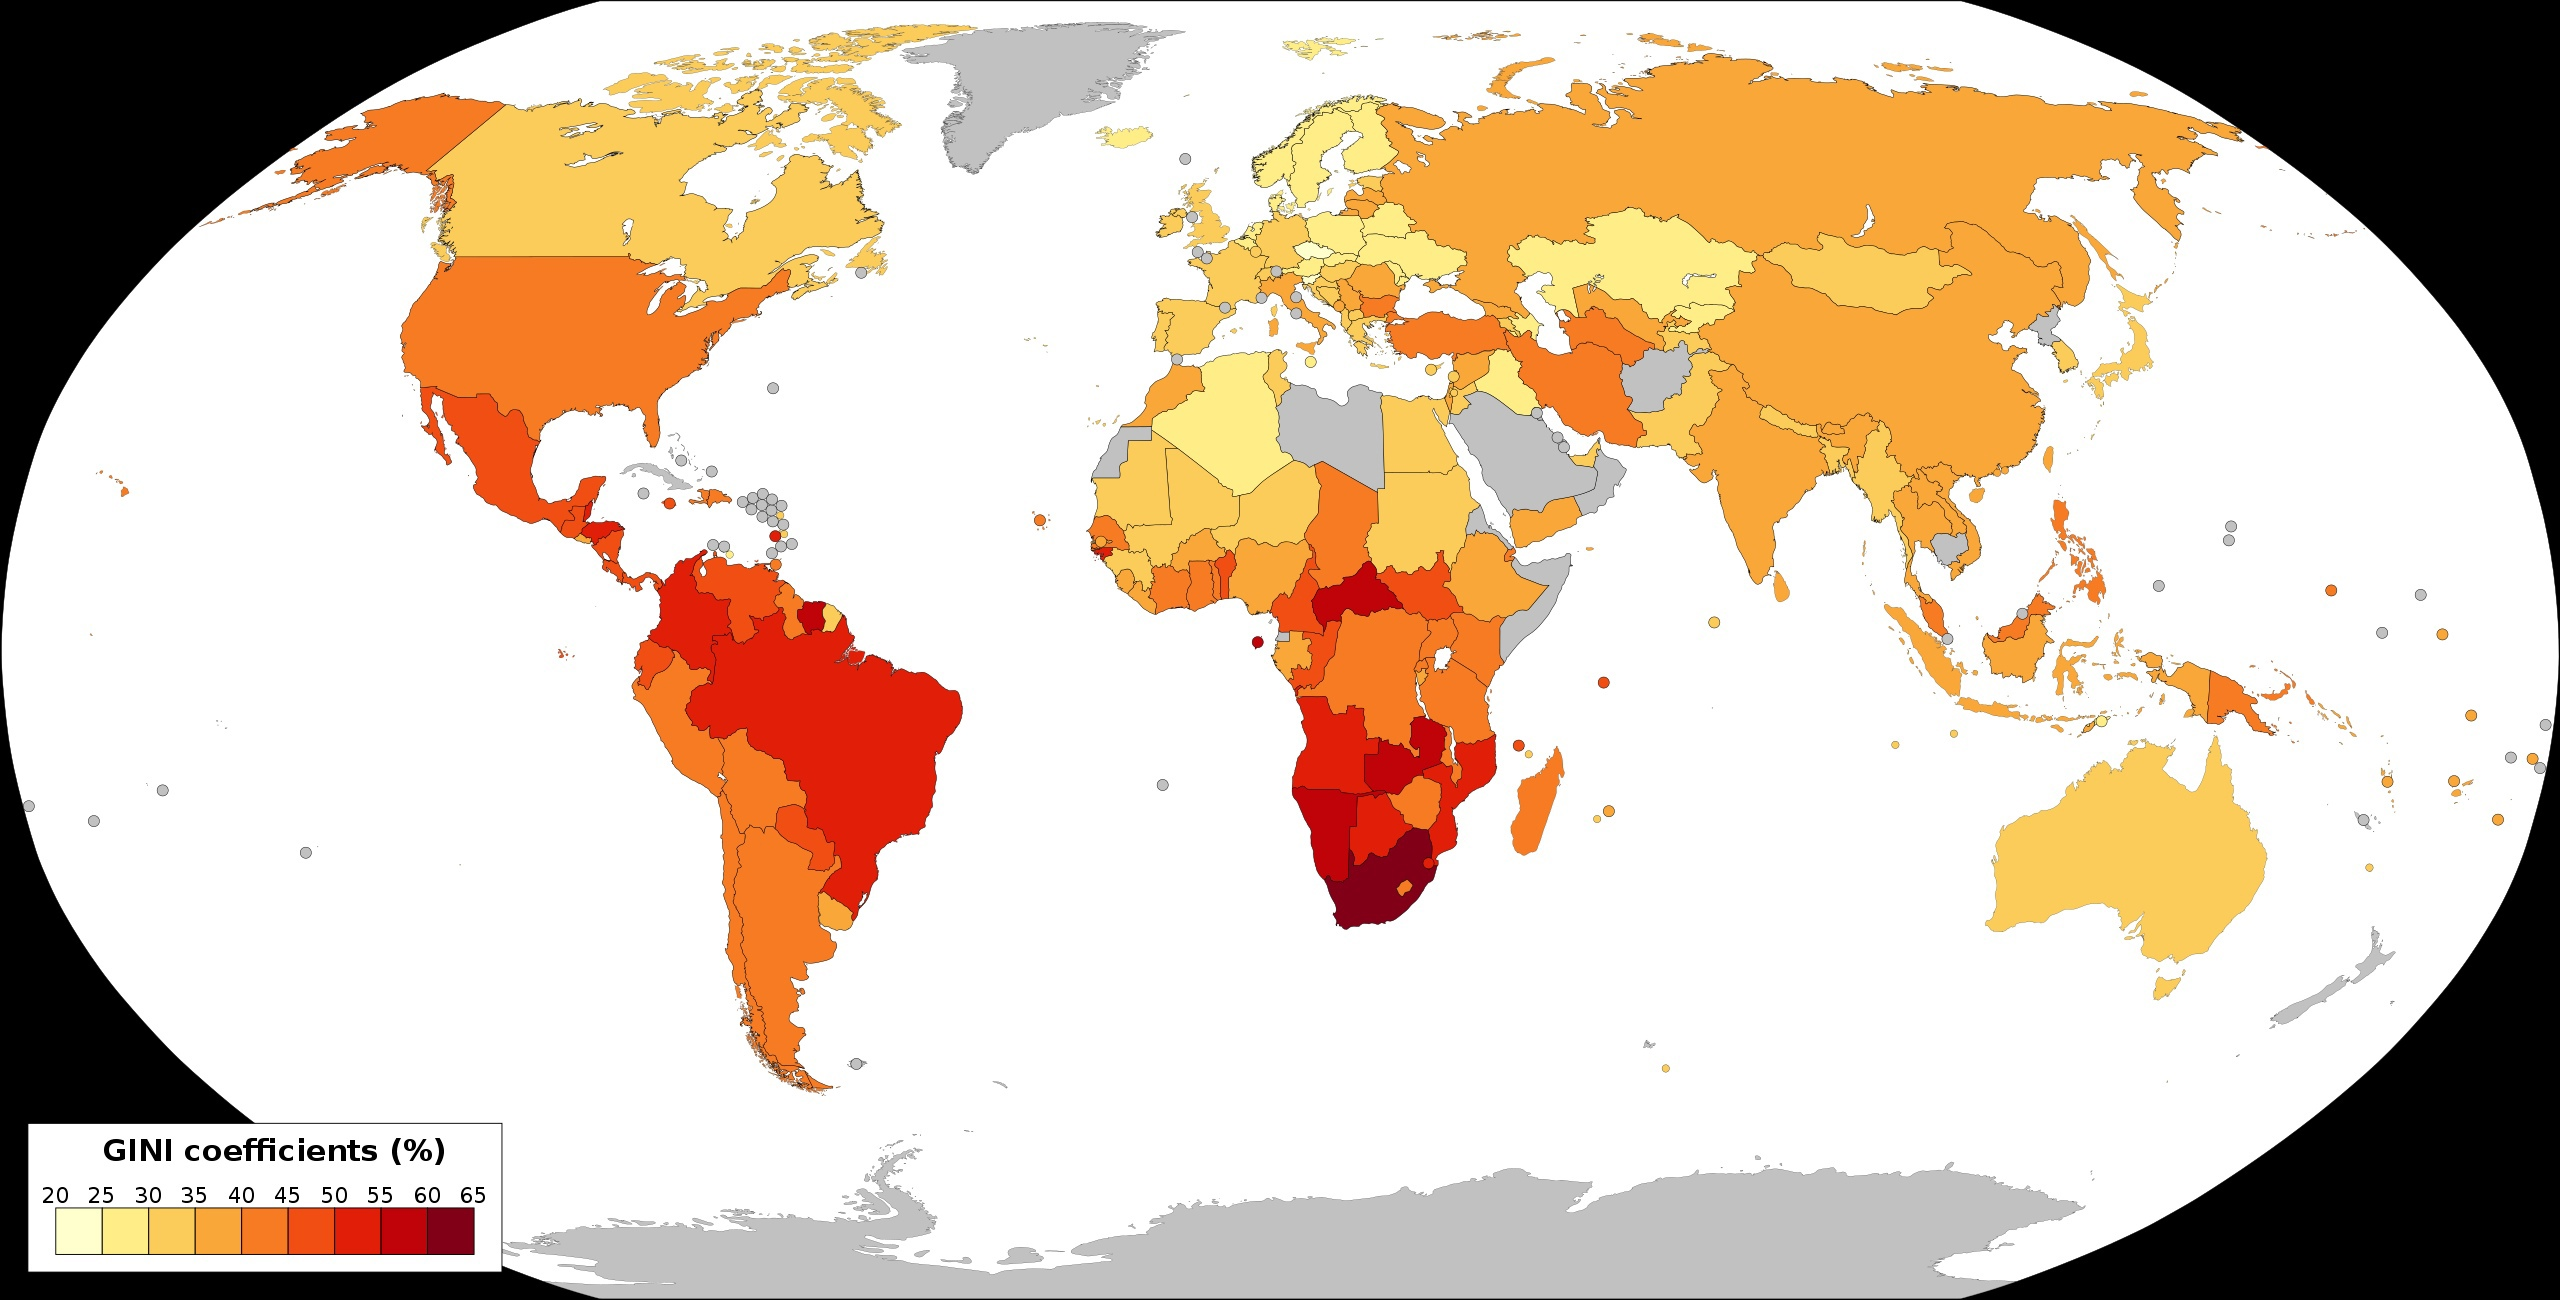
\includegraphics[width=0.75\textwidth]{gini_index_world.jpg}
    \caption{Индекс Джини по странам мира}
\end{figure}
Даже в ЮАР индекс Джини составляет 57.8\%.

    \section{Дальнейшее развитие}\label{sec:todo}
    Несмотря на то, что программа уже работоспособна, есть ещё много идей и планов по её усовершенствованию:


 \subsection{Внедрить \textit{быстрый пересчёт функции ошибки}}
Это улучшение давно напрашивается,
но оно несколько теряет в эффективности из-за того, что в одной мутации в среднем изменяется
не так мало мазков (однако это количество убывает со временем).
В настоящий момент ведётся работа над внедрением.

\subsection{Разделение мазков по слоям}
 Нетрудно заметить, что при рисовании картин художники сначала проходятся по холсту черновыми мазками большого размера, а затем — прорабатывают детали.
 Таких уровней детализации зачастую бывает немало.

 Пример того, как художник (\href{https://www.youtube.com/watch?v=VaXHtai2alU}{https://www.youtube.com/watch?v=VaXHtai2alU}) рисует картину по слоям:

\begin{figure}[h!]
    \centering
    \subfloat{\includegraphics[width=0.24\textwidth]{painting_example_layer_0.png}}
    \subfloat{\includegraphics[width=0.24\textwidth]{painting_example_layer_1.png}}
    \subfloat{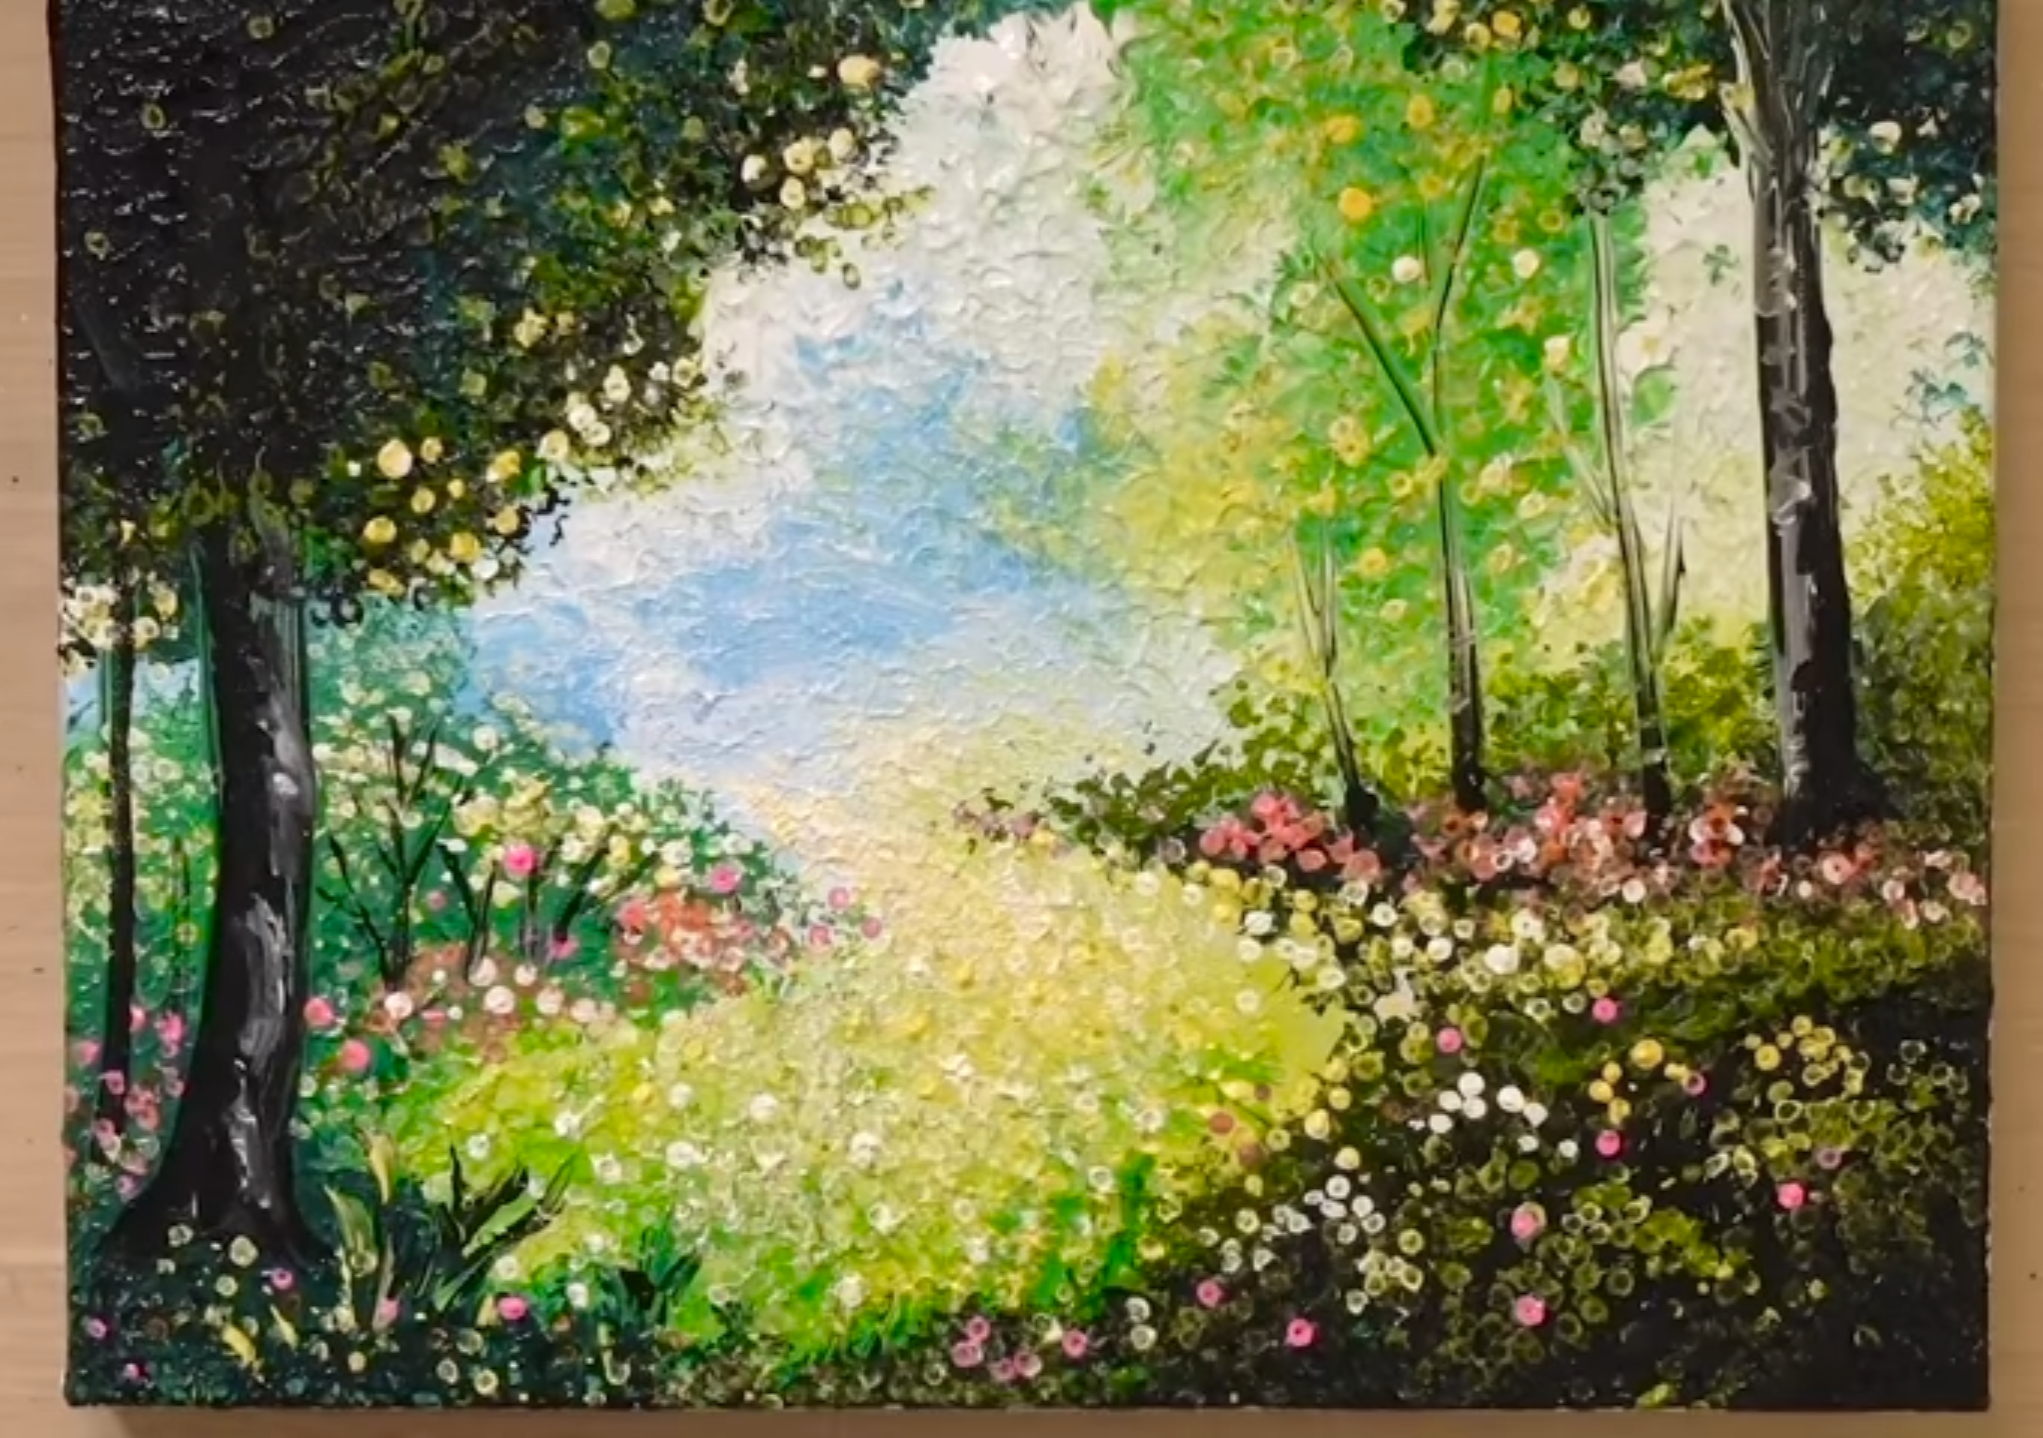
\includegraphics[width=0.24\textwidth]{painting_example_layer_2.png}}
    \subfloat{\includegraphics[width=0.24\textwidth]{painting_example_layer_3.png}}
    \caption{ Фон | Рельеф фона | Детализация заднего плана | Основные объекты}
    \label{fig:layered_painting}
\end{figure}


Поэтому стоит попробовать сначала заполнять картинку толстыми, грубыми мазками
(то есть просто с большей шириной, а в реальной жизни это будет отражаться в большем размере кисти и в более сильном нажатии).

\subsection{Добавить возможность использования локальных методов оптимизации}
Такие методы, как \textbf\textit{{градиентный спуск}} и \textbf\textit{{метод Ньютона}} позволяют достичь гораздо большей скорости сходимости
(в случае метода ньютона — сходимость \href{http://w.ict.nsc.ru/books/textbooks/akhmerov/mo_unicode/4.html}{квадратичная}),
но требуют умения посчитать градиент функции ошибки в любой точке, а также вектор вторых производных по каждому из аргументов.

Сами алгоритмы реализованы и находятся в \href{https://github.com/donRumata03/PowerfulGA/blob/master/other_optimization/local_optimization.cpp}{этой папке}.
Предусмотрена опция подсчёта первой и вторых производных через подстановку близких значений параметров:

\begin{equation}
    f'(x_0) \approx \frac{f(x_0 + \Delta x) - f(x_0)}{\Delta x}
\end{equation}

Однако в случае с мазками при маленьких изменениях параметров функция ошибки остаётся неизменной, так как это приводит к такому же набору закрашенных пикселей.
Соответственно, нужно либо радикально увеличивать разрешение изображения, либо использовать аналитические методы.
То есть нужно математически посчитать изменение функции ошибки при бесконечно малом изменении из параметров функции.

 \subsection{Организовать систему тестирования различных алгоритмов на различных функциях}\label{itm:testing_system}
Звучит как нечто весьма простое, но реальность сложнее, чем кажется.
Напрашивающийся вариант — дать каждому алгоритму заданное количество вычислений функции ошибки и сравнить, какой результат они получат.

Однако функция ошибки нелинейная, поэтому сложно будет понять,
насколько сильному различию в качестве алгоритма соответствует полученная численная разница в результатах.

Целесообразно сравнивать количество итераций, требующееся алгоритмам для получения заданного результата.
Но и тут не всё так просто: нельзя просто запустить алгоритмы на неограниченное количество итераций
и ждать дотижения нужного значения функции,
так как во многих из них (как минимум — в моей модификации ГА) то,
как будет проведена каждая отдельная итерация, сильно зависит от процента выполнения на момент её прохождения:
происходит планирование,  использующее информацию о максимальном количестве итераций.


Поэтому нет никакого другого выхода, кроме того, чтобы запускать этот алгоритм с рахым количеством итераций и смотреть, когда он в среднем будет доходить до заданного порога.
Это необходимо автоматизировать.
В идеальном случае для поиска порога можно было бы использовать бинарный поиск, но в реальности (с поправкой на шум) имеет смысл использовать эвристическую модификацию н-арного поиска (объяснить!).
Для полной оценки планируется построить график достаточного количества итераций от nребуемого значения функции в интересующей нас зоне.

\subsection{Улучшить алгоритм поиска цветов и разделения на зоны}\label{subsec:posterisation_and_zoning}

Сейчас для разделения изображения на зоны используется Adobe Illustrator.
По заданному количеству цветов (и, следовательно, уровню детализации) он разделяет изображение на зоны,
присваивая каждой какой-то из цветов палитры так, чтобы он хорошо .
Сама палитра тоже формируется в ходе работы алгоритма.

Скорее всего, для этого используется один из популярных алгоритмов, описанных \href{https://en.wikipedia.org/wiki/Color_quantization}{здесь}, или некая проприетарная их вариация.
Зоны, на которые происходит деление, описываются частями плоскости, ограниченными кривыми безье — «path»  формате $svg$.
Несмотря на то что формально алгоритм выполняет свою работу, большое количество зон имеет очень продолговатую форму,
а также наблюдается неимоверный разброс в размерах между разными зонами (см. \ref{subsec:inequality}):
всё это уменьшает эффективность процесса.

% TODO: написать про свой алгоритм и склеивание зон

\subsection{Перенести графические вычисления на видеокарту}\label{subsec:move_graphics_to_videocard}
Также напрашивающееся улучшение.
Это может существенно ускорить работу алгоритма, особенно — генетического (так как при нём можно распараллелить вычисление для целой популяции),
причём только в случае, если не используется быстрый пересчёт функции ошибки или мутирует очень много мазков одновременно.
Как бы то ни было, когда-нибудь стоит добавить эту возможность.
Тестовый проект с использованием OpenCL я уже написал.

Изначальная картинка будет переноситься в видеопамять один раз — в начале работы программы.
Выделить память для матрицы можно также один раз, а потом каждый раз её очищать (эту операцию можно производить параллельно).

Если использовать видеокарту для распараллеливания вычислений, встаёт вопрос, на каком именно уровне производить разделение.
Варианты такие:
\begin{enumerate}
    \item Каждое изображение — на своём потоке.
    Такой способ подходит только для ГА в случае огромного размера поколения (так как потоков у видеокарты порядка нескольких тысяч).
    Для отжига — никогда.

    \item Каждый мазок — на своём потоке.
                Тут возникают проблемы с синхронизацией, так как порядок наложения важен: как минимум не должны появляться в хаотическом порядке пиксели из мазков разного цвета.
                Даже если происходит смешение цветов при наложении, синхронизация важна.
                Это можно сделать через дополнительную струкрутру данных в виде прямоугольной матрицы, в которой для каждого пикселя будет записываться список цветов с приоритетами
                (индексами мазков, а значит, и числами, определяющими порядок слоёв).
                Потом уже независимо для каждого пикселя будет происходить обработка смешения или наложения с замещением «попавших» на него цветов.
                Всё упирается в умение синхронизировать потоки.
                Тут нужно либо симуляцию мьютекса для каждого пикселя (то есть матрицу булевых значений «занят-не занят»),
                либо умение распределить мазки по потокам так, чтобы в каждый момент времени не было никаких двух с накладывающимися bounding-box'ами.

                В первом случае либо нужно покупать видеокарту с поддержкой атомарных значений, либо придётся вставлять дополнительные проверки,
                чтобы два потока не прочитали почти одновременно состояние «не занят»  и не зашли туда до того, как какой-либо из них успеет записать состояние «закрыто».

                Во втором случае уменьшится количество потоков, одновременно работающих над одной «картиной».


    \item Проводить распараллеливыание на графическом примитиве нисшего уровня, использующемся в данном алгоритме (см. \ref{subsec:rasterization}).
                Например, полигоны или круги.
                Видеокарта умеет эффективно отрисовывать такие примитивы.
                Однако количество точек в примитивах обычно невелико: существенно меньше, чем ядер в видеокарте.
\end{enumerate}
Причём всегда можно комбинировать разделения на разных уровнях.

Когда будет произведена растеризация, на той же видеокарте посчитается функция ошибки: в этом случае легко сделать это независимо для каждого пикселя.
Единственное — нужно помнить, что для добавления наказания за наложения и пустоты в функцию ошибки надо составлять дополнительные матрицы, в которых это будет указано.


Адаптация алгоритмов под видеокарту описана здесь: \ref{subsec:rasterization}.

\end{document}